% -*- TeX-master: "tccudesc.tex" -*-
\chapter{O gerador de código}
\label{cap3}

Dada uma especificação na linguagem \TLAA, contendo elementos da lógica TLA e da teoria de conjuntos, além de elementos sintáticos próprios, deseja-se obter uma definição equivalente em linguagem de programação. Equivalência para esse propósito é definida pela igualdade do conjunto de comportamentos permitidos. Isto é, todo comportamento especificado deve ser permitido na execução do código, e todo comportamento permitido pela execução do código deve ter sido especificado.

\section{Elixir}
\label{elixir}

Para esse propósito, a linguagem de programação escolhida para o código traduzido foi Elixir. As motivações são expostas abaixo por ordem de relevância na decisão:
\begin{enumerate}
  \item A concorrência é facilitada por ter seu código traduzido para \textit{bytecode} da máquina virtual do Erlang (BEAM). Suporte a concorrência é de extrema importância, já que \TLA foi criado para facilitar a especificação de sistemas concorrentes. É necessário que o código gerado seja capaz de refletir o sistema também nesse quesito.

  \item Uma linguagem funcional tende a se(setq mouse-wheel-scroll-amount '(1 ((shift) . 1) ((control) . nil)))  aproximar mais de definições matemáticas do que linguagens de outros paradigmas. Uma vez que a estrutura de \TLA foi construída principalmente no âmbito da matemática, a complexidade das traduções tende a ser menor para uma linguagem funcional.

  \item O alto nível de abstração da sintaxe de Elixir, que se inspira em Ruby e sua busca por código facilmente entendível, faz com o programador que trabalhar com o código gerado possa entendê-lo de forma mais simples e rápida do que seria com uma linguagem de baixo nível. Com isso, otimizações podem ser feitas com mais segurança, e a manutenabilidade do código é favorecida.

  \item A transparência de plataforma provida pela máquina virtual BEAM maximiza o número de ambientes aonde o código pode ser executado. Não seria de muito uso gerar um código para um ambiente específico, e uma máquina virtual permite que o código gerado seja \textit{cross plataform}.

  \item O seu código é aberto sobre a licença Apache 2.0, permitindo que o funcionamento de suas estruturas possa ser verificado a qualquer momento. Não seria possível garantir nenhuma correspondência do código gerado com a especificação se não fosse conhecida a execução gerada pelos operadores usados no código.

\end{enumerate}

Essa escolha vem de encontro com a finalidade de proporcionar um código modificável, de forma que o programador seja capaz de entender a correspondência entre as duas partes e minimizando a diferença do nível de abstração no qual ele está programando.

\section{A tradução}
\label{traducao}

A geração de código para uma especificação se dá pela tradução das estruturas de \TLA para Elixir. Esta tradução será feita de forma automática por uma ferramenta escrita em Haskell, implementada durante o corrente trabalho. A ferramenta será responsável pelo \textit{parsing} do aquivo da especificação, no formato \texttt{.tla}, para estruturas internas e, então, transformação dessas estruturas internas em código Elixir.

A escolha da linguagem Haskell para implementação do gerador de código é motivada pela possibilidade da definição de tipos algébricos, que facilitam na representação das estruturas, e na tipagem forte, que ajuda a garantir consistência das relações entre estruturas definidas durante o processo, minimizando a possibilidade de erros no desenvolvimento. Haskell também conta com a biblioteca de \textit{parsing} Parsec, que abstrai a complexidade de analisar sintaticamente um arquivo.

O escopo da tradução se limita à especificação definida, sendo suficiente para gerar código executável para o sistema definido. Traduzir teoremas e suposições não é necessário, uma vez que essas estruturas servem para fazer verificações sobre a especificação e não são necessárias para seu funcionamento. Ao código gerado não é atribuída a responsabilidade de refazer verificações, e sim de manter as propriedades já verificadas.

\subsection{Mapeamentos}
\label{mapeamentos}

A tradução funciona como um grande mapeamento do conjunto de todas as especificações para um conjunto de programas em Elixir. Para viabilizar esse mapeamento, são definidos sub-mapeamentos que traduzem frações de uma especificação. Encontrar sub-mapeamentos suficientes para atender todo o domínio de especificações é suficiente para definir o processo de tradução.

Os primeiros mapeamentos definidos envolvem fórmulas transicionais e variáveis. Para cada fórmula transicional da especificação, é definida uma função, declarada com a sintaxe \texttt{def nome(parametros) do ... end}, que recebe as variáveis como parâmetro. O conjunto de variáveis do sistema é representado em uma Hash - estrutura de dados chave-valor de Elixir, equivalente a um dicionário - representada no padrão \texttt{variaveis = \%\{ variavel1: valor1, variavel2: valor2 \}} e podendo ser acessada com \texttt{variaveis[:variavel1]} para obter \texttt{valor1}.

Cada função mapeada de uma ação recebe uma hash representando o estado atual e retorna outra hash representando o novo estado. O retorno, em Elixir, não exige uma palavra chave - a função retorna aquilo que a última linha retornou, sendo, para as funções geradas, a hash resultante da chamada do seu construtor.

A Figura \ref{fig:esvaziapequeno-elixir} contém a função mapeada da fórmula $EsvaziaPequeno$ definida na Figura \ref{fig:ex1tla}.

\begin{figure}[h]
  \centering
  $\progfig{
  ~~def esvazia\_pequeno(variaveis) do\\
  ~~~~\%\{\\
  ~~~~~~pequeno: 0,\\
  ~~~~~~grande: variaveis[:grande]\\
  ~~~~\}\\
  ~~end
  }$
  \caption{Fórmula transicional $EsvaziaPequeno$ como uma função em Elixir}
\label{fig:esvaziapequeno-elixir}
\end{figure}

Alguns operadores de \TLA permitem mapeamentos ainda mais diretos, como \IF e \CASE, devido a sua inspiração em linguagens de programação. A Figura \ref{fig:pequenoparagrande-elixir} traz a função correspondente à fórmula $PequenoParaGrande$ definida na Figura \ref{fig:ex1tla}. A sintaxe para operadores \IF em Elixir é na forma \texttt{if condição do ... else ... end}.

\begin{figure}[h]
  \centering
  $\progfig{
  ~~def pequeno\_para\_grande(variaveis) do\\
  ~~~~if variaveis[:grande] + variaveis[:pequeno] <= 5 do\\
  ~~~~~~\%\{\\
  ~~~~~~~~pequeno: 0,\\
  ~~~~~~~~grande: variaveis[:grande] + variaveis[:pequeno]\\
  ~~~~~~\}\\
  ~~~~else\\
  ~~~~~~\%\{\\
  ~~~~~~~~pequeno: variaveis[:pequeno] - (5 - variaveis[:grande]),\\
  ~~~~~~~~grande: 5\\
  ~~~~~~\}\\
  ~~~~end\\
  ~~end
  }$
  \caption{Fórmula transicional $PequenoParaGrande$ como uma função em Elixir}
\label{fig:pequenoparagrande-elixir}
\end{figure}

Com o conjunto inicial de mapeamentos apresentado, é possível definir todas as fórmulas transicionais do sistema definido na Seção \ref{exemplo1}. Ao traduzir as definições $Init$ e $Next$, é possível executar concorrentemente todos os comportamentos permitidos pela especificação. A definição $Next$ é traduzida para a função \texttt{main}, que recebe as variáveis para o estado atual e dispara um processo para cada passo permitido por $Next$. Como $Next$ é uma disjunção de todas as ações, é disparado um novo processo com o resultado de cada função traduzida.

Para disparar processos, é chamada a função da biblioteca padrão de Elixir responsável por executar processos ligados: \texttt{spawn\_link}. Essa função é chamada com três parâmetros: o módulo que receberá a chamada, a função a ser executada e uma lista contendo seus parâmetros. Para a tradução de $Next$, o módulo é sempre o módulo do arquivo gerado (\texttt{JarrosDeAgua}), a função é sempre \texttt{main} e os parâmetros são o resultado da aplicação de um dos passos permitidos. O último disparo corresponde à aplicação de um passo balbuciante. A definição dessa função encontra-se na Figura \ref{fig:main-ex1}.

\begin{figure}[h]
  \centering
  \progfig{
  ~def main(variaveis) do\\
  ~~~spawn\_link JarrosDeAgua, :main, [grande\_para\_pequeno(variaveis)]\\
  ~~~spawn\_link JarrosDeAgua, :main, [pequeno\_para\_grande(variaveis)]\\
  ~~~spawn\_link JarrosDeAgua, :main, [esvazia\_grande(variaveis)]\\
  ~~~spawn\_link JarrosDeAgua, :main, [esvazia\_pequeno(variaveis)]\\
  ~~~spawn\_link JarrosDeAgua, :main, [enche\_grande(variaveis)]\\
  ~~~spawn\_link JarrosDeAgua, :main, [enche\_pequeno(variaveis)]\\
  ~~~spawn\_link JarrosDeAgua, :main, [variaveis]\\
  ~end\\\\
  ~JarrosDeAgua.main(\%\{\ grande: 0, pequeno: 0 \})
  }
  \caption{Disparo de processos para o sistema de Jarros de Água}
\label{fig:main-ex1}
\end{figure}

A chamada \texttt{JarrosDeAgua.main(\%\{grande: 0, pequeno: 0\})} é a tradução de $Init$. Como esse sistema permite um único estado inicial, apenas uma chamada a \texttt{main} é necessária. Com ela, todos os passos dados para iniciar novos processos terão iniciado com o valor para variáveis que satisfaz a condição inicial. Através da definição de \texttt{main}, é também garantido que todos os passos satisfazem $\square [Next]_{vars}$. Assim, todos os comportamentos iniciados com essa chamada são permitidos por $Spec$, conforme definida na Seção \ref{exemplo1}.

O código gerado para esse sistema não permite, por si só, a solução do problema - uma vez que a especificação não tratava de uma solução. Entretanto, verificou-se que a invariante $jarro\_grande\ \backslash= 4$ não é satisfeita, e portanto um comportamento que leva à solução é permitido por esse sistema. É possível, apenas para fins exploratórios, encontrar os processos disparados pelo código que correspondem a esses comportamentos. Para isso, uma chamada que encerra o programa é invocada se o predicado da invariante for insatisfeito. Essa verificação é feita em todos os passos do comportamento, e portanto é definida como uma condição na função \texttt{main} como na Figura \ref{fig:invariant-ex1}, que imprime os valores das variáveis com \texttt{IO.puts} e encerra o programa com um código de sucesso através de \texttt{:ok}.

\begin{figure}[h]
  \centering
  $\progfig{
  ~def main(variaveis) do\\
  ~~~if variaveis[:grande] == 4 do\\
  ~~~~~IO.puts "\#\{variaveis[:grande]\} \#\{variaveis[:pequeno]\}"\\
  ~~~~~:ok\\
  ~~~end\\
  ~~~\dots\\
  ~end
  }$
  \caption{Exploração de invariantes no código gerado}
\label{fig:invariant-ex1}
\end{figure}

Com essa tradução inicial, é evidenciada a semelhança entre as definições
matemáticas de \TLA e as estruturas do paradigma funcional presentes em Elixir.
Entretanto, o disparo de múltiplos processos contemplando todos os caminhos
possíveis do sistema não é viável dada a explosão de estados nem possui
aplicação prática de muito valor. Assim, se apresenta a maior dificuldade
encontrada durante o desenvolvimento deste trabalho: como traduzir
especificações intermediárias que não descrevem uma implementação e sim um
sistema ou protocolo.

A tradução da especificação completa de uma implementação não resultaria no
disparo de múltiplos processos pela definição $Next$ porque, ao especificar uma
implementação, são definidas quais condições levam a execução de cada ação. Isso
é evidenciado pela comparação das especificações do sistema (Figura
\ref{fig:ex2tla}), do protocolo e da implementação no Capítulo \ref{cap2}. Como o
intuito do gerador de código é fornecer um protótipo funcional e viável, e não
um disparador de processos interminável, são necessárias condições bem definidas
para a decisão de que ação deve ser tomada. A Seção \ref{sec:condicoes}
descreve como a exigência dessas condições é feita.

\subsection{Condições e Ações}
\label{sec:condicoes}

Na definição de uma ação em \TLAA, existem expressões de estado e expressões de
ação (descritas na seção \ref{sec:tla}). As expressões de estado em uma ação
\FANCYA são predicados que terão valoração verdadeira se e somente se o estado em que \FANCYA
será executada - ou seja, o primeiro estado do passo - seja um estado onde
\FANCYA é permitido. Essas expressões, quando dentro da definição de uma ação,
podem ser interpretadas como condições de ativação dessa ação. A ação só pode ser ativada
se suas condições de ativação forem satisfeitas.

Já uma expressão de ação envolve ambos os estados de um passo - o estado atual e
o próximo estado. Se tratada puramente como uma especificação, esse próximo
estado pode ser entendido como qualquer estado possível especificado, de forma
que, de todos os estados possíveis, a expressão de ação só será verdadeira para
aqueles pares de estado que respeitam a condição por ela determinada. Com essa
perspectiva, as expressões de ação também são condições.

Contudo, no contexto de um programa executável viável, os estados são obtidos de
maneira incremental. No código gerado, o estado inicial é obtido pela definicão
do estado inicial da especificação, e os próximos estados são obtidos a partir
da sucessiva aplicação de funções - que representam ações - nesse estado.

Gerar todos os estados possíveis e avaliar uma ``condição de ação'' para cada um dos
passos para então filtrá-los seria uma forma possível de executar o programa, porém
não é viável quando há muitos valores possíveis para as variáveis de estado. Ao
especificar $x' = x + 1$, define-se que todos os pares de estado onde o segundo estado tem o
valor de $x$ igual ao valor $x - 1$ do primeiro estado. Contudo, em uma
implementação, gerar pares de estado que para todos os valores
inteiros e filtrar os que atendem essa condição é
inviável. Nesse contexto, é possível simplesmente gerar os pares de estado válidos e,
considerando que o estado atual é conhecido durante a execução, isso significa apenas
somar 1 ao valor de $x$ para obter o segundo estado do par que satisfaz a ação.

As expressões de ação, no código gerado proposto, são operações efetuadas sobre
um estado que resultam sempre em um novo estado válido. Para isso, elas só são
ativadas quando as condições de ativação (definidas pelas expressões
de estado) são satisfeitas. A divisão
entre expressões de estado, que serão transformadas em condições, e expressões de
ação, que serão transformadas em funções que alteram o estado, é feita pelo
próprio parser já que essas expressões se distinguem na gramática da linguagem
de \TLAA.

\begin{figure}[h]
  \centering
  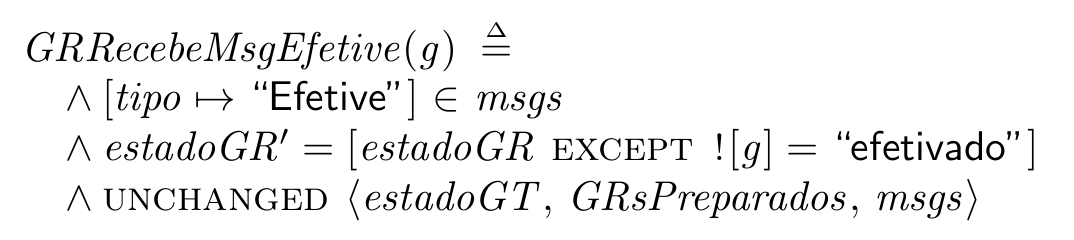
\includegraphics[width=0.8\textwidth]{GRRecebeMsgEfetive.png}
  \caption{Ação para o recebimendo da mensagem ``Efetive'' por um gerenciador de
  recurso}
  \label{fig:recebe-efetive-tla}
\end{figure}
\begin{figure}[h]
  \centering
  $\progfig{
  def gr\_recebe\_msg\_efetive\_condition(variables, g) do\\
  ~~Enum.member?(variables[:msgs], \%\{tipo: "Efetive"\})\\
  end\\\\

  def gr\_recebe\_msg\_efetive(variables, g) do\\
  ~~\%\{\\
  ~~~~estado\_gr: Map.put(variables[:estado\_gr], g, "efetivado"),\\
  ~~~~estado\_gt: variables[:estado\_gt],\\
  ~~~~grs\_preparados: variables[:grs\_preparados],\\
  ~~~~msgs: variables[:msgs]\\
  ~~\}\\
  end\\
  }$
  \caption{Código gerado para a ação $GRRecebeMsgEfetive(g)$}
\label{fig:recebe-efetive-elixir}
\end{figure}


Na especificação do protocolo de efetivação em duas fases, na Figura
\ref{fig:ex3tlap2}, o tradutor transformara cada uma das ações em duas funções:
uma de retorno booleano determinando se a condição de ativação é satisfeita, e
outra retornando o estado resultante da aplicação da ação. A Figura
\ref{fig:recebe-efetive-tla} é um recorte dessa especificação, e será traduzida
nas duas funções expostas na Figura \ref{fig:recebe-efetive-elixir}.


\subsection{Determinando a próxima ação}
\label{sec:decisao}

Como discutido na Seção \ref{sec:protocolo}, a ação de próximo estado $Next$
pode ser atendida por mais de um próximo estado $t$ para o mesmo estado atual $s$.
Isso não é um problema para o TLC, que avalia todos os pares estados possíveis distintos
que atendem as condições da ação, verificando todas as ramificações da árvore de
estados. No programa gerado, contudo, executar uma ação significa fazer possivelmente uma alteração de estado, e
múltiplas alterações de estado não são interessantes para o propósito do
código gerado, conforme discutido na Seção \ref{mapeamentos}.

Assim, é necessário um processo bem definido para decidir qual ação executar a
partir de um estado. Para garantir que seja possível tomar tais decisões sem uma
situação que exija uma escolha, é
necessário que a especificação defina, para cada estado do comportamento, condições de ativação mutualmente
exclusivas para ações disjuntas com próximos estados distintos - isto é,
sempre que há uma disjunção de ações, para todos os estados de um comportamento,
todas as condições de ativação dessas ações devem ser falsas para aquele estado exceto pelas daquelas
que levem ao próximo estado do comportamento.

Uma especificação que atenda essa restrição descreve uma função pura, onde não
há efeitos colaterais e uma mesma entrada, dada pelo estado inicial, sempre gera uma mesma
saída, dada pelo comportamento - sequência de estados - obtido. \TLA permite,
contudo, especificar diversos comportamentos válidos a partir do mesmo estado
inicial, o que possibilita que a sequência de estados possa ser eventualmente modificada por
efeitos colaterais e permanecer válida.

Para garantir que o comportamento satisfaz a especificação, as influências de
efeitos colaterais devem obedecer a função de próximo estado. Isso quer dizer
que as influências são, para cada estado da execução, a escolha de uma ação que
satisfaça a função de próximo estado. Como o estado atual $s$ já é conhecido em
tempo de execução, a influência precisa levar a um estado $t$ tal que $<s,t>$
satisfaça tal função.

Quando é definido o conceito de escolha na Seção \ref{sec:protocolo}, define-se que é possível
que exista apenas um valor possível para $t$ que atenda essa restrição. Isso acontece quando a restrição
de condições de ativação mutualmente exclusivas é respeitada pelo estado atual.
Nesse caso, a influência externa não é necessária, já que é possível decidir o
valor de $t$. Assim, a influência externa só é necessária quando uma escolha é
exigida. Nesses casos, o código gerado estabelece uma troca de mensagens entre o
processo gerado pelo modelo e um novo processo denominado oráculo, que será
responsável por toda influência externa no modelo.

O Algoritmo \ref{alg:decide-action} é responsável por examinar as ações
possíveis e decidir qual será aplicada ao estado atual - seja por uma decisão
pura ou por uma escolha de um influência externa. Ela recebe uma identificação
da ação origem, isto é, a definição cuja disjunção de ações precisa de uma
decisão; e uma lista de ações que contém, para cada ação, um rótulo, o valor da
sua condição de ativação para o estado atual e o próximo estado que sua execução traria.

\begin{algorithm}
\caption{Decisão da próxima ação}\label{alg:decide-action}
\begin{algorithmic}[1]
\Procedure{DecideAção}{origem, ações}
\State $acoes\_possiveis\gets$ ações com condição satisfeita
\State $estados\_distintos\gets$ estados únicos resultantes de $acoes\_possiveis$
\If{tamanho de $estados\_distintos=1$}\Comment{Decisão pura}
\State \textbf{return} primeiro estado em $estados\_distintos$
\Else\Comment{Influência Externa}
\State envie identificações das $acoes\_possiveis$ para o oráculo
\State $acao\_escolhida\gets$ resposta do oráculo
\State \textbf{return} estado resultante de $acao\_escolhida$
\EndIf
\EndProcedure
\end{algorithmic}
\end{algorithm}

Se há apenas um próximo estado possível resultante das aplicações das ações
ativadas, então o algoritmo decide por aquele estado. Caso contrário, ele abre
uma conexão com o oráculo, enviando uma identificação das ações
possíveis. O algoritmo permanece bloqueado até que o oráculo responda a ação
escolhida, e então retorna o próximo estado correspondente àquela ação.


\subsection{Concorrência}

Mesmo \TLA sendo uma linguagem de especificação para sistemas concorrentes, ela
não permite descrições para um \textit{fork} ou disparo de novos
processos. O valor de \TLA para sistemas concorrentes é possibilitar um conjunto
de ordens de execução válido, e não limitar a apenas uma única ordem. Sistemas
concorrentes usualmente apresentam muitos comportamentos distintos, e \TLA
permite especificar um modelo que aceite vários desses comportamentos.

Assim, o modelo em si e sua tradução são sequenciais, e se comportam como uma troca
sucessiva de estados. A ordem das transições que alteram esses estados é
possivelmente determinada por uma influência externa - e esta, sim, pode possuir
elementos concorrentes.

Considerando o sistema dos Jarros de Água do Capítulo \ref{cap2}, cada passo da
execução exige uma escolha, já que nenhuma ação tem condição de ativação. Uma
forma de fazer essa escolha é através do disparo de vários processos onde cada
um seleciona uma das possíveis ações - esses processos podem ser representados
como pessoas com intenções diferentes de resolver o problema dos jarros. Não é
possível permitir que mais de uma pessoa (ou processo) altere o estado dos
jarros ao mesmo tempo. É possível, contudo, a partir de uma fila ou de uma
escolha aleatória de pessoas, estabelecer uma ordem de ações sobre os jarros.

Algumas operações computacionais, como a escrita em um endereço de memória,
serializam ações - já que não podem ser feitos concorrentemente. Isso não
significa que essas operações não precisam ser levadas em conta quando usadas em
um sistema concorrente. Elas são justamente o ponto onde podem ocorrer problemas
nesse tipo de sistema, nos momentos onde processos paralelos precisam de um
recurso compartilhado e a ordem em que eles o obtém influencia o resultado
final. Por isso, um procedimento de serialização como a ordem de obtenção de um
recurso compartilhado pode acontecer de várias maneiras diferentes, e em razão
disso sua especificação é importante.

Um exemplo mais tangível desse fenômeno pode ser dado pelo protocolo de
efetivação em duas fases, discutido na Seção \ref{sec:protocolo}, onde existem vários gerenciadores de recursos
enviando suas intenções de efetivar ou abortar para um gerenciador de transações
compartilhado entre eles. O gerenciador de transações é um processo sequencial,
mas pode ter vários comportamentos diferentes devido as possíveis ordens que as
mensagens dos gerenciadores de recurso chegam.

\section{Regras de Tradução}
\label{sec:regras}

A partir de especificação escritas em \TLAA conforme a sintaxe da figura
\ref{fig:notacao-tla}, deseja-se obter um código executável em Elixir com
elementos da Figura \ref{fig:notacao-elixir}. As regras de tradução são
divididas em camadas conforme a recursão das definições, de forma que a
especificação completa é traduzida no código pelas regras $\vdash$.


\begin{figure}[h]
  \centering
  \fbox{\[\begin{array}{l} \begin{array}{lrllll}
    \text{Identificadores} & I, k & ~~~~
    \text{Valores} & v & ~~~~ \text{Parâmetros} & p \\
    \end{array} \\ \\
    \begin{array}{lrcl}
      \text{Especificação} & Spec & ::= & Module M\\
      &&&\CONSTANTS C_o, \dots, C_n\\
      &&&\VARIABLES\ V_o, \dots, V_n\\
      &&&NomeAcao_0(p_{00}, \dots, p_{0n}) \triangleq \FANCYA_0\\
      &&&\vdots\\
      &&&NomeAcao_n(p_{n0}, \dots, p_{nn}) \triangleq \FANCYA_n\smallskip\\
  \text{Definição} & \FANCYA & ::= & A \,\mid\, P \,\mid\, \FANCYA \land
                                \FANCYA \,\mid\, \FANCYA \lor \FANCYA \smallskip\\
  \text{Predicado} & P, Q & ::= & \neg P \,\mid\, P \land P \,\mid\, P \lor P
                                  \,\mid\, v_1 \in v_2 \,\mid\, v_1 = v_2\\
                                  &&\,\mid\,& v_1 \neq v_2 \,\mid\, \ENABLED \FANCYA\smallskip\\
  \text{Ação} & A & ::= & I' = v \,\mid\, \UNCHANGED \langle I_0, \dots, I_n \rangle\smallskip\\
  \text{Conjunto} & S & ::= & {v} \,\mid\, S_a \cup S_b\smallskip\\
  \text{Registro} & R & ::= & [k \mapsto v] \,\mid\, [I \EXCEPT ![k] = v]\smallskip\\
  \end{array} \end{array}\]}
  \caption{Sintaxe aceita para \TLA}
\label{fig:notacao-tla}
\end{figure}

\begin{figure}[h]
  \centering
  \fbox{\[\begin{array}{l} \begin{array}{lrllll}
    \text{Átomos} & \tti , \ttk & ~~~~
    \text{Valores} & \ttx , \tty & ~~~~ \text{Parâmetros} & \ttp \\
    \end{array} \\ \\
    \begin{array}{lrcl}
  \text{Estado} & \tta & ::= & \texttt{nome\_acao(variables, $\ttp_0$, ..., $\ttp_n$)} \,\mid\, \texttt{variables}\\
      &&\,\mid\,& \texttt{\%\{ $\tti_o : \ttx_o$, ..., $\tti_n : \ttx_n$ \}} \,\mid\, \texttt{Map.merge(a, a)} \smallskip\\
  \text{Condição} & \ttc & ::= &  \texttt{nome\_acao\_condition(variables,
                              $\ttp_0$, ..., $\ttp_n$)}\\
                              &&\,\mid\,& \texttt{not c} \,\mid\, \texttt{c and c} \,\mid\,
                              \texttt{c or c}\smallskip\\
  \text{Conjunto} & \tts & ::= & \texttt{MapSet.new([x])} \,\mid\, \texttt{MapSet.union($\tts_a$, $\tts_b$)}\smallskip\\
  \text{Registro} & \ttr & ::= & \texttt{\%\{ k: x \}} \,\mid\, \texttt{Map.put(i,
                              k, x)}\smallskip\\
  \text{Definição} & \texttt{def} & ::= & \texttt{def nome\_acao(variables,
                                          $\ttp_0$, ..., $\ttp_n$)}\\
      &&\,\mid\,& \texttt{def\_decide\_action}\ (\text{\small vide Algoritmo \ref{alg:decide-action}}) \smallskip\\
  \end{array} \end{array}\]}
  \caption{Elementos gerados em Elixir}
\label{fig:notacao-elixir}
\end{figure}



Em \TLAA, as definições \FANCYA englobam predicados e ações e, como discutido na
Seção \ref{sec:condicoes}, deseja-se separá-los em condições \ttc\ e ações sobre
os estados \tta. Devido a essas definições com misturas de predicados e ações
serem recursivas, é necessário que haja uma separação recursiva também. Para
isso, ao traduzir uma definição com as regras $\vdash_d$, utiliza-se uma
estrutura intermediária na forma de dupla, contendo uma lista das condições
recursivamente encontradas e traduzidas como primeiro elemento, e das ações como
segundo.

Além das traduções especificadas nas regras desta seção, o gerador de código
também carrega os comentários da especificação, transformando comentários que
antecedem as definições em documentação através das anotações \texttt{@doc} do
Elixir. Também são omitidas das regras traduções básicas de expressões
aritméticas e alguns detalhes implementados para melhorar a legibilidade do
código gerado, como identação e conversão de \textit{casing}. 

A Seção \ref{sec:validacao} apresenta exemplos de aplicação das regras
apresentadas nesta seção, e por isso é possivelmente um recurso para melhor
compreendimento do funcionamento do tradutor. Por questão organizacional, as
regras e exemplos são mantidos em seções distintas, mas recomenda-se a
referência entre eles no momento da leitura deste capítulo.

\subsection{Tradução de especificações}

	\begin{figure}[H]
	\centering
  {\fbox{
      $\begin{array}{c}

         \fbox{$\vdash Spec \TEq code$} \\ \\

      \begin{array}{c}
          \begin{minipage}[t]{0.6\textwidth}
           \infer[\text{\tt (MOD)}]{
             \begin{array}{l}
               \Gamma\vdash
               \begin{array}{l}
                 \MODULE\ M\\
                 \CONSTANTS\ C_0, \dots, C_n\\
                 \VARIABLES\ V_0, \dots, V_n\\
                 Def_0\\
                 \vdots\\
                 Def_n\\
                 Def_{init}\\
                 Def_{next}
             \end{array}
               \TEq
               \progfigmed{
               defmodule M do\\
               ~~@oracle spawn(Oracle, :listen, [])\\
               ~~$\texttt{const}_0$, ..., $\texttt{const}_n$\\
               ~~$\texttt{def}_0$, ..., $\texttt{def}_n$\\
               ~~def\_next\\
               ~~def\_decide\_action\\
               end\\\\
               M.main(state)}
             \end{array}
           }
           {
             \begin{array}{c}
               \Gamma\vdash \CONSTANTS C_0, \dots, C_n \TEq \texttt{$\texttt{const}_0$, ..., $\texttt{const}_n$}\smallskip\\
               \begin{array}{rll}
                 \Gamma \cup \{C_0 : const, \dots, C_n : const\} \vdash& Def_0 &\TEq \texttt{def}_0\\
                 \vdots&\\
                 \Gamma \cup \{C_0 : const, \dots, C_n : const\} \vdash& Def_n &\TEq \texttt{def}_n\smallskip\\
                 \Gamma \cup \{C_0 : const, \dots, C_n : const\} \vdash_{next}& Def_{next} &\TEq \texttt{def\_next}\smallskip\\
                 \Gamma \cup \{M : module, C_0 : const, \dots, C_n : const\} \vdash_{init}& Def_{init} &\TEq \texttt{state}
               \end{array}
             \end{array}
           }
         \end{minipage}\vspace*{.7cm}\\

        \begin{minipage}[t]{0.8\textwidth}
          \infer[\text{\tt (DEF)}]{
            \begin{array}{c}
              \Gamma\vdash NomeAcao(p_0, \dots, p_n) \triangleq \FANCYA \TEq\\
              \progfig{
              def nome\_acao\_condition(variables, $p_0,\ \dots,\ p_n$)\ do\\
              ~~$c_0$\ and \ ...\ and\ $c_n$\\
              end\\
              def nome\_acao(variables, $p_0,\ \dots,\ p_n$)\ do\\
              ~~Map.merge($a_0$, Map.merge(..., $a_n$))\\
              end
              }
            \end{array}
          }
          {
            \Gamma \cup \{p_0 : param, \dots, p_n : param\} \vdash_d \FANCYA \TEq ((c_o, \dots,
            c_n), (a_0, \dots, a_n))
          }
        \end{minipage}\vspace*{.7cm}\\

        \begin{minipage}[t]{0.8\textwidth}
          \infer[\text{\tt (CONST)}]{
            \Gamma\vdash\CONSTANTS C_0, \dots, C_n \TEq
            \begin{array}{c}
              \progfigsmall{
              @$C_0$ ``<Value for $C_0$>''\\
              def $C_0$, do:\ @$C_0$\\
              $\vdots$\\
              @$C_n$ ``<Value for $C_n$>''\\
              def $C_n$, do:\ @$C_n$
              }
            \end{array}
          }
          {
          }
        \end{minipage}\\

      \end{array}
			\end{array}$
		}}
		\caption{Tradução da especificação}
		\label{fig:t-specification}
	\end{figure}



A tradução de uma especificação para código Elixir é dada pela regra
(\texttt{MOD}) na Figura\ref{fig:t-specification}.
O julgamento $\vdash$ é responsável pelo início da tradução, recebendo a
especificação completa e traduzindo cada elemento com o julgamento devido.
A partir dela, um módulo Elixir é obtido, assim como a invocação de sua
função \texttt{main} com o estado inicial traduzido. Dentro do módulo, o oráculo
é disparado e referenciado por uma constante, as constantes são declaradas e as
definições traduzidas formam o restante das funções, juntamente com a função de
próximo estado e a função \texttt{decide\_action} definida pelo Algoritmo \ref{alg:decide-action}.

As definições declaradas são traduzidas pela regra (\texttt{DEF}) (Figura
\ref{fig:t-declaration}) que, a partir das duplas
obtidas recursivamente de uma definição \FANCYA, cria as funções \texttt{nome\_acao\_condition} 
e \texttt{nome\_acao}, reduzindo as condições com o conector lógico \texttt{and}
e as ações com a função \texttt{merge}, responsável por unificar duas
estruturas do tipo \texttt{Map} - usada para representar estados - em uma só.

A declaração de constantes é traduzida pela regra (\texttt{CONST}), que define,
para cada constante declarada na especificação, um atributo do módulo gerado em
Elixir, a partir do operador \texttt{@}, assim como uma função que permite acessá-la de
fora do módulo. O valor das constantes em \TLA só precisa ser definido para
executar o TLC, e não está presente na especificação. Assim, o código gerado
atribui um valor exemplo da forma ``<Value for C>'' a ser substituído pelo programador.


\subsection{Tradução das definições}

As definições de ações e predicados é recursivamente agregada em uma dupla de
listas. Os predicados encontrados são traduzidos para condições com pelas regras
$\vdash_P$ em (\texttt{COND}) e agregados na primeira lista da dupla, enquanto as ações são
traduzidas em funções sobre o estado pelas regras $vdash_a$ em (\texttt{ACT}) e agregadas na
segunda lista.

Quando uma definição é invocada dentro de outra definição, como acontece com
$podeEfeitvar$ e $naoEfetivado$ na especificação de transações em bancos de
dados na Figura \ref{fig:ex2tla} e em nas definições de próximo estado apresentadas, aplica-se a regra
$(\texttt{CALL})$, que adiciona a condição e a ação daquela definição às
respectivas listas, incorporando completamente a definição invocada.


\begin{figure}[h]
	\centering
  {\fbox{
      $\begin{array}{c}

         \fbox{$\Gamma\vdash_d \FANCYA \TEq (\overline{c}, \overline{a})$} \\\\
         \begin{array}{c}
         \begin{minipage}[t]{0.8\textwidth}
           \infer[\text{\tt (CALL)}]{
             \begin{array}{c}
               \Gamma\vdash_d NomeAcao(v_0, \dots, v_n)
               \TEq\\ (\{\texttt{\small nome\_acao\_condition(variables, $\ttx_0$, ...,
               $\ttx_n$)}\},\\
               \{\texttt{\small nome\_acao(variables,
                 $\ttx_0$, ..., $\ttx_n$)}\})
             \end{array}
           }
           {
             \begin{array}{c}
               \Gamma\vdash_v v_0 \TEq x_0\\
               \vdots\\
               \Gamma\vdash_v v_n \TEq x_n
             \end{array}
           }
         \end{minipage}\vspace{.7cm}\\

           \begin{minipage}[T]{0.2\textwidth}
           \infer[\text{\tt (COND)}]{
             \Gamma\vdash_d P \TEq (\{c\},\ \{\})
           }
           {
             \Gamma\vdash_p P \TEq c
           }\vspace*{.7cm}

           \infer[\text{\tt (ACT)}]{
             \Gamma\vdash_d A \TEq (\{\},\ \{a\})
           }
           {
             \Gamma\vdash_a A \TEq a
           }

         \end{minipage}\hspace*{.7cm}

           \begin{minipage}[B]{0.5\textwidth}
           \infer[\text{\tt (IF-DIRECT)}]{
               \Gamma\vdash_d
             \begin{array}{l}
               \IF P\\
               \THEN \FANCYA_t\\
               \textsc{ else}\ \FANCYA_e
             \end{array}
             \TEq (\{\},\ \{action\})
           }
           {
             \begin{array}{c}
               \Gamma\vdash_p P \TEq c\\
               \Gamma\vdash_d \FANCYA_t \TEq (\{\},\ \{\texttt{at}_0, \dots, \texttt{at}_n\})\\
               \vdots\\
               \Gamma\vdash_d \FANCYA_e \TEq (\{\},\ \{\texttt{ae}_0, \dots, \texttt{ae}_n\})\\
             \end{array}
           }
         \end{minipage}\vspace{.7cm}\\

         \begin{minipage}[t]{0.5\textwidth}
           \infer[\text{\tt (IF-COND)}]{
               \Gamma\vdash_d
             \begin{array}{l}
               \IF P\\
               \THEN \FANCYA_t\\
               \textsc{ else}\ \FANCYA_e
             \end{array}
             \TEq (\{condition\},\ \{action\})           }
           {
             \begin{array}{c}
               \Gamma\vdash_p P \TEq c\\
               \Gamma\vdash_d \FANCYA_t \TEq (\{\texttt{ct}_0, \dots, \texttt{ct}_n\},\ \{\texttt{at}_0, \dots, \texttt{at}_n\})\\
               \vdots\\
               \Gamma\vdash_d \FANCYA_t \TEq (\{\texttt{ce}_0, \dots, \texttt{ce}_n\},\ \{\texttt{ae}_0, \dots, \texttt{ae}_n\})\\
             \end{array}
           }
         \end{minipage}\vspace*{-0.5cm}\\

           \begin{minipage}[t]{0.5\textwidth}
             \hspace*{-2cm}
             \begin{array}{l}
               onde\\
               condition =\\\\\\\\\\\\
               action =\\\\\\\\
             \end{array}
             \progfigmed{\\\\
               if c do\\
               ~~$\texttt{ct}_0$ and ... and $\texttt{ct}_n$\\
               else\\
               ~~$\texttt{ce}_0$ and ... and $\texttt{ce}_n$\\
               end\\\\
                 if c do\\
                 ~~Map.merge($\texttt{at}_0$, Map.merge(..., $\texttt{at}_n$))\\
                 else\\
                 ~~Map.merge($\texttt{ae}_0$, Map.merge(..., $\texttt{ae}_n$))\\
                 end
               }
           \end{minipage}\\
         \end{array}
			\end{array}$
		}}
		\caption{Tradução intermediária de definições - Geração}
		\label{fig:definitions}
	\end{figure}

\begin{figure}[h]
	\centering
  {\fbox{
      $\begin{array}{c}

         \fbox{$\Gamma\vdash_d \FANCYA \TEq (\overline{c}, \overline{a})$} \\\\
         \begin{array}{c}

         \begin{minipage}[B]{0.5\textwidth}
           \infer[\text{\tt (AND)}]{
               \Gamma\vdash_d
               \begin{array}{c}
                 \land\ \FANCYA_0 \\
                 \vdots \\
                 \land\ \FANCYA_n
               \end{array}
               \TEq (\overline{c_o} \cup \dots \cup \overline{c_n},\ \overline{a_o} \cup \dots \cup \overline{a_n})
           }
           {
             \begin{array}{c}
               \Gamma\vdash_d \FANCYA_0 \TEq (\overline{c_0},\ \overline{a_0})\\
               \vdots\\
               \Gamma\vdash_d \FANCYA_n \TEq (\overline{c_n},\ \overline{a_n})
             \end{array}
           }
         \end{minipage}\vspace{.7cm}\\
           \begin{minipage}[t]{0.8\textwidth}
             \infer[\text{\tt (OR)}]{
                 \begin{array}{l}
                   \Gamma\vdash_d
                   \begin{array}{c}
                     \lor\ \FANCYA_0 \\
                     \vdots \\
                     \lor\ \FANCYA_n
                   \end{array}
                   \TEq (\{\},\ \{\text{\tt decide\_action}(l)\})
                 \end{array}
               }
               {
                 \begin{array}{c}
                   \Gamma\vdash_d \FANCYA_0 \TEq (\{c_{00}, \dots, c_{0n}\},\ \{\ a_{00}, \dots, a_{0n}\})\\
                   \vdots\\
                   \Gamma\vdash_d \FANCYA_n \TEq (\{c_{n0}, \dots, c_{nn}\},\ \{a_{n0}, \dots, a_{nn}\})\\
               \end{array}
             }
         \end{minipage}\\

           \begin{minipage}[t]{0.8\textwidth}
             \hspace*{2cm}
             \progfigmed{
               $onde\ l =$
               [\\
               ~~\%\{\\
               ~~~~action: show([$a_{00}, \dots, a_{0n}$])\\
               ~~~~condition: $c_{00}$\ and\ $\dots$\ and\ $c_{0n}$\\
               ~~~~state: Map.merge($a_{00}$, Map.merge($\dots$, $a_{0n}$))\\
               ~~\},\\
               ~~$\dots$,\\
               ~~\%\{\\
               ~~~~action: show([$a_{n0}, \dots, a_{nn}$])\\
               ~~~~condition: $c_{n0}$\ and\ $\dots$\ and\ $c_{nn}$\\
               ~~~~state: Map.merge($a_{n0}$, Map.merge($\dots$, $a_{nn}$))\\
               ~~\}\\
               ]\\
             }\vspace*{-1cm}

           \end{minipage}
         \end{array}
			\end{array}$
		}}
		\caption{Tradução intermediária de definições - Agregação}
		\label{fig:definitions}
	\end{figure}


\subsubsection{Condicionais}

Estruturas \IF definem ações com base em uma condição, e poderiam ser traduzidas
para a disjunção de duas definições com suas próprias condições e ações, de forma que uma das
definições tenha a condição idêntica a condicional de \IF e a outra, sua
negação. A as ações seriam enviadas para o algoritmo de decisão, já que se
encontram em uma disjunção, mas nunca precisariam de uma escolha uma vez que a
condicional torna suas condições mutualmente excludentes.

Para não adicionar
indireções possivelmente confusas e preservar a semelhança com a especificação, contudo, optou-se por utilizar
a própria estrutura \texttt{if} da linguagem destino. As definições dos blocos
\IF e \textsc{else} podem conter tanto condições quanto ações, porém essas não
podem ser mantidas em uma mesma expressão \texttt{if}, já que é necessário
avaliar as condições antes de aplicar as ações. A expressão obtida da ação deve
sempre resultar em uma alteração de estado, e no caso do \texttt{if}, a alteração
dependente de uma condicional. Para que sempre haja o retorno de um novo estado, é necessário avaliar as
condições antes e não durante a ação, e para uma essa ação \IF ser ativável, é necessário
atender as condições de ativação da definição em
\THEN se a condicional for verdadeira, e as condições de ativação de \textsc{else} caso
a condicional seja falsa - ou seja, a condição de ativação também depende da
condicional. Assim, a regra (\texttt{IF}) gera duas estruturas \texttt{if}, uma
para as condições e outra para as ações

\subsubsection{Agregação}

\begin{figure}[h]
	\centering
  {\fbox{
      $\begin{array}{c}

         \fbox{$\Gamma\vdash_d \FANCYA \TEq (\overline{c}, \overline{a})$} \\\\
         \begin{array}{c}

         \begin{minipage}[B]{0.5\textwidth}
           \infer[\text{\tt (AND)}]{
               \Gamma\vdash_d
               \begin{array}{c}
                 \land\ \FANCYA_0 \\
                 \vdots \\
                 \land\ \FANCYA_n
               \end{array}
               \TEq (\overline{c_o} \cup \dots \cup \overline{c_n},\ \overline{a_o} \cup \dots \cup \overline{a_n})
           }
           {
             \begin{array}{c}
               \Gamma\vdash_d \FANCYA_0 \TEq (\overline{c_0},\ \overline{a_0})\\
               \vdots\\
               \Gamma\vdash_d \FANCYA_n \TEq (\overline{c_n},\ \overline{a_n})
             \end{array}
           }
         \end{minipage}\vspace{.7cm}\\
           \begin{minipage}[t]{0.8\textwidth}
             \infer[\text{\tt (OR)}]{
                 \begin{array}{l}
                   \Gamma\vdash_d
                   \begin{array}{c}
                     \lor\ \FANCYA_0 \\
                     \vdots \\
                     \lor\ \FANCYA_n
                   \end{array}
                   \TEq \left(\{\},\ \{
                   \begin{array}{c}
                   \progfigmed{
                     decide\_action(List.flatten[\\
                     ~~$\ttinfo_0$,\\
                     ~~...,\\
                     ~~$\ttinfo_n$\\
                     ])}\}
                   \end{array}\right)
                 \end{array}
               }
               {
                 \begin{array}{c}
                   \Gamma\vdash_i \FANCYA_0 \TEq \ttinfo_0\\
                   \vdots\\
                   \Gamma\vdash_i \FANCYA_n \TEq \ttinfo_n\\
               \end{array}
             }
         \end{minipage}\\
         \end{array}
			\end{array}$
		}}
		\caption{Tradução intermediária de definições - Agregação}
		\label{fig:definitions}
	\end{figure}

\begin{figure}[h]
	\centering
  {\fbox{
      $\begin{array}{c}

         \fbox{$\Gamma\vdash_i \FANCYA \TEq \texttt{info}$} \\\\
         \begin{array}{c}

           \begin{minipage}[t]{0.8\textwidth}
             \infer[\text{\tt (INFO-DEF)}]{
                   \Gamma\vdash_i
                     \FANCYA 
                   \TEq
                   \begin{array}{c}
                     \progfigmed{
                     \\\%\{\\
                     ~~action: show([$a_0, \dots, a_n$])\\
                     ~~condition: $c_0$\ and\ $\dots$\ and\ $c_n$\\
                     ~~state: Map.merge($a_0$, Map.merge($\dots$, $a_n$))\\
                     \},\\
                     }
                   \end{array}
               }
               {
                 \begin{array}{c}
                   \Gamma\vdash_d \FANCYA \TEq (\{c_0, \dots, c_n\},\ \{\ a_0, \dots, a_n\})\\
               \end{array}
             }
         \end{minipage}\\

           \begin{minipage}[B]{0.5\textwidth}
           \infer[\text{\tt (INFO-EX)}]{
                 \begin{array}{c}
               \Gamma\vdash_d
               \exists I \in v : \FANCYA_0 \lor \dots \lor \FANCYA_n
               \TEq
                 \begin{array}{l}
                   \texttt{\small Enum.map(x, fn (i) -> [}\\
                   \ \ \ \ \ttinfo_0,\\
                   \ \ \ \ \texttt{...}\\
                   \ \ \ \ \ttinfo_n\\
                   \ \ \texttt{]}\\
                   \texttt{end}
                \end{array}
                \end{array}
           }
           {
             \begin{array}{c}
               \Gamma\vdash_v v \TEq x\\
               \Gamma\vdash_i \FANCYA_0 \TEq \ttinfo_0\\
               \vdots\\
               \Gamma\vdash_i \FANCYA_n \TEq \ttinfo_n\\
             \end{array}
           }
         \end{minipage}\vspace{.7cm}\\

         \end{array}
			\end{array}$
		}}
		\caption{Organização das informações sobre uma ação}
		\label{fig:definitions}
	\end{figure}


Quando as definições são conectadas pelo E lógico ($\land$), aplica-se a regra
(\texttt{AND}) e as listas de
condições e ações para cada definição são concatenadas - essas listas serão
devidamente reduzidas a um elemento válido em outras regras.

Já quando o conector é o OU lógico ($\lor$), é necessário iniciar o processo de decisão
discuto nas Seções \ref{sec:protocolo} e \ref{sec:decisao}. A regra
(\texttt{OR}) não gera nenhuma nova condição, e encapsula o processo de decisão
em uma única ação que se dá pela invocação da função \texttt{decide\_action},
que implementa o Algoritmo \ref{alg:decide-action} e retorna a ação que deve ser
executada. Essa função recebe uma lista com três informações para cada definição conectada
pelo OU, que são geradas pelas regras do julgamento $\vdash_i$.

Dada uma definição, a regra (\texttt{INFO-DEF}) gera uma estrutura \texttt{Map}
com: Uma identificação da definição (gerada por uma função \texttt{show} de
conversão da estrutura para \texttt{string}); A redução das condições
encontradas na definição; e a redução das ações. Entre as definições a serem
enviadas para o algoritmo de decisão, é possível que haja um quantificador
existencial, determinando definições com parâmetros dependentes
de algum valor. Nesse caso, a regra (\texttt{INFO-EX}) define uma chamada para a
função \texttt{map}, que será capaz de gerar as informações conforme os valores
em tempo de execução.


\subsubsection{Tradução de Predicados}

Os predicados em \TLA são fórmulas sobre o estado atual, e são traduzidos para
expressões lógicas sobre o estado denominadas condições, e estarão sempre
associados a execução de uma ação. As traduções são bem diretas e mapeiam os
operadores de igualdade, desigualdade e pertence para suas representações em
Elixir.

\begin{figure}[h]
	\centering
  {\fbox{
      $\begin{array}{c}

         \fbox{$\Gamma\vdash_p P \TEq c$} \\ \\

         \begin{array}{c}
           
         \begin{minipage}[t]{0.25\textwidth}
           \infer[\text{\tt (PRED-EQ)}]{
               \Gamma\vdash_p v_x = v_y \TEq \texttt{x == y}
           }
           {
             \Gamma\vdash_v v_x \TEq x\hspace*{.4cm}
             \Gamma\vdash_v v_y \TEq y
           }
         \end{minipage}\hspace*{.2cm}
           
         \begin{minipage}[t]{0.25\textwidth}
           \infer[\text{\tt (PRED-NEQ)}]{
               \Gamma\vdash_p v_x \noteq v_y \TEq \texttt{x != y}
           }
           {
             \Gamma\vdash_v v_x \TEq x\hspace*{.4cm}
             \Gamma\vdash_v v_y \TEq y
           }
         \end{minipage}\vspace*{.7cm}\\

         \begin{minipage}[t]{0.4\textwidth}
           \infer[\text{\tt (PRED-IN)}]{
               \Gamma\vdash_p v_e \in v_l \TEq \texttt{Enum.member?($l$,\ $e$)}
           }
           {
             \Gamma\vdash_v v_e \TEq e\hspace*{.4cm}
             \Gamma\vdash_v v_l \TEq l
           }
         \end{minipage}\\
         \end{array}\vspace*{1cm}\\

         \fbox{$\Gamma\vdash_a A \TEq a$} \\ \\

         \begin{array}{c}
           
         \begin{minipage}[t]{0.6\textwidth}
           \infer[\text{\tt (ACT-UNCH)}]{
         \begin{array}{c}
             \Gamma\vdash_a \UNCHANGED \langle I_0, \dots, I_n \rangle \TEq\\
             \texttt{\%\{ $I_0$:\ variables[:$I_0$]$,\ \dots,\ I_n$:\ variables[:$I_n$] \}}
         \end{array}
           }
           {
           }
         \end{minipage}\vspace*{.7cm}\\

         \begin{minipage}[t]{0.4\textwidth}
           \infer[\text{\tt (ACT-PRIM)}]{
               \Gamma\vdash_a I' = v \TEq \texttt{\%\{ $I$:\ $x$ \}}
           }
           {
             \Gamma\vdash_v v \TEq x
           }
         \end{minipage}\\
         \end{array}
			\end{array}$
		}}
		\caption{Tradução de predicados e ações}
		\label{fig:t-pred-act}
	\end{figure}
  


\subsubsection{Tradução de Ações}

As ações definidas em \TLA são fórmulas envolvendo o próximo estado. Em elixir,
os estados são representados com a estrutura chave-valor \texttt{Map} em um parâmetro chamado \texttt{variables}, e uma
ação traduz para uma nova estrutura desse tipo. Assim, ao aplicar a regra (\texttt{ACT-UNCH}) para uma ação do
tipo \UNCHANGED - isto é, o valor da variável no próximo estado permanece o
mesmo - a nova estrutura indica que o valor para aquela chave, que representa a
variável, é o valor que a estrutura anterior tinha para tal chave. A
estrutura anterior é obtida pelo parâmetro \texttt{variables}, e o valor referente à
chave \tti é obtido por \texttt{variables[:i]}.

De forma semelhante, quando há uma modificação do valor da variável na transição
de estado, indicado pelo operador \textit{primed}, a tradução é feita pela regra
(\texttt{ACT-PRIM}) e a estrutura para o próximo estado apresenta o
novo valor para a chave referente à variável sendo modificada.

Nas regras $\vdash_a$, cada ação de \TLA é transformada em uma estrutura do tipo
\texttt{Map}. Essas estruturas são posteriormente agregadas com a função
\texttt{merge}, que teriam um formato como \texttt{Map.merge(variables, Map.merge(\%\{ i: 1 \}, \%\{
  j: 2 \}))}. Para melhorar a legibilidade, após a tradução, o gerador agrega os
valores literais em uma única estrutura, de forma que esse mesmo estado fica
representado como \texttt{Map.merge(variables, \%\{ i: 1, j: 2 \})}.

\subsubsection{Tradução de valores}

\begin{figure}[h]
	\centering
  {\fbox{
      $\begin{array}{c}

         \fbox{$\Gamma\vdash_p P \TEq c$} \\ \\

         \begin{array}{c}
           
         \begin{minipage}[t]{0.25\textwidth}
           \infer[\text{\tt (PRED-EQ)}]{
               \Gamma\vdash_p v_x = v_y \TEq \texttt{x == y}
           }
           {
             \Gamma\vdash_v v_x \TEq x\hspace*{.4cm}
             \Gamma\vdash_v v_y \TEq y
           }
         \end{minipage}\hspace*{.2cm}
           
         \begin{minipage}[t]{0.25\textwidth}
           \infer[\text{\tt (PRED-NEQ)}]{
               \Gamma\vdash_p v_x \noteq v_y \TEq \texttt{x != y}
           }
           {
             \Gamma\vdash_v v_x \TEq x\hspace*{.4cm}
             \Gamma\vdash_v v_y \TEq y
           }
         \end{minipage}\vspace*{.7cm}\\

         \begin{minipage}[t]{0.4\textwidth}
           \infer[\text{\tt (PRED-IN)}]{
               \Gamma\vdash_p v_e \in v_l \TEq \texttt{Enum.member?($l$,\ $e$)}
           }
           {
             \Gamma\vdash_v v_e \TEq e\hspace*{.4cm}
             \Gamma\vdash_v v_l \TEq l
           }
         \end{minipage}\\
         \end{array}\vspace*{1cm}\\

         \fbox{$\Gamma\vdash_a A \TEq a$} \\ \\

         \begin{array}{c}
           
         \begin{minipage}[t]{0.6\textwidth}
           \infer[\text{\tt (ACT-UNCH)}]{
         \begin{array}{c}
             \Gamma\vdash_a \UNCHANGED \langle I_0, \dots, I_n \rangle \TEq\\
             \texttt{\%\{ $I_0$:\ variables[:$I_0$]$,\ \dots,\ I_n$:\ variables[:$I_n$] \}}
         \end{array}
           }
           {
           }
         \end{minipage}\vspace*{.7cm}\\

         \begin{minipage}[t]{0.4\textwidth}
           \infer[\text{\tt (ACT-PRIM)}]{
               \Gamma\vdash_a I' = v \TEq \texttt{\%\{ $I$:\ $x$ \}}
           }
           {
             \Gamma\vdash_v v \TEq x
           }
         \end{minipage}\\
         \end{array}
			\end{array}$
		}}
		\caption{Tradução de predicados e ações}
		\label{fig:t-pred-act}
	\end{figure}


O mapeamento de valores é a camada mais baixa da tradução, e está bastante
ligada a sintaxe. Conjuntos são traduzidos pra estruturas do tipo
\texttt{MapSet}, que armazenam valores únicos em árvores binárias de busca;
Registros são traduzidos para estruturas chave-valor \texttt{Map}, variáveis
são acessadas pelo estado disponível no parâmetro \texttt{variables} e
constantes pelo atributo do módulo.

Para decidir como traduzir um identificador, que pode representar uma variável,
uma constante ou um parâmetro da de definição, utiliza-se o contexto $\Gamma$.
Se o contexto indicar que um identificador é um parâmetro, ele é traduzido sem
modificação.

Se ele for uma constante, é necessário verificar se a tradução está
sendo solicitada de uma definição de dentro do módulo ou de fora - como é no
caso da tradução do estado inicial. Se o contexto não tiver informação do
módulo, significa que essa tradução vem de dentro do próprio módulo e então a
constante pode ser acessada como uma constante do módulo, através do prefixo
\texttt{@}. Caso haja uma indicação de módulo, é necessário traduzi-la para a
chamada da função de acesso à constante daquele módulo, através de
\texttt{NomeDoModulo.constante}.

Se o identificador não for nem um parâmetro e nem uma constante, então ele
representa uma variável do estado e pode ser acessado por \texttt{variables[:i]}.

\subsection{Estado Inicial}

Para verificar propriedades no TLC, o \TLA exige uma definição dos estados
iniciais possíveis. Essa definição tem a forma de um predicado sobre um estado
- e não um passo - ou seja, não é uma ação.

Ao definir o predicado sobre estados iniciais para enviá-lo ao TLC, é
possivelmente desejável que mais de um estado atenda-o, de forma que o TLC
inicie a exploração do espaço de estados a partir de mais de um estado. Isso
traria segurança de que, independentemente de quais dos estados iniciais definidos o
programa se encontre no momento que inicia, seu comportamento será válido.

No contexto da execução desse programa, considera-se que não há benefício em
permitir mais de um possível estado inicial. Uma possibilidade de lidar com uma
definição de múltiplos estados iniciais seria delegar a escolha do estado
inicial ao oráculo, porém isso significaria uma interação com o oráculo antes do
início da execução do modelo, sendo que, nesse momento, o programador poderia
fazer a escolha de forma mais simples. Assim, opta-se por encarregar o
programador de definir o predicado para estados iniciais de forma a garantir que
haja apenas um possível estado que satisfaça-o.

Após a ferramenta de tradução ser aplicada em contextos diferentes, será
possível observar de que forma o oráculo é utilizado pelos programadores.
Considera-se que se for comum o oráculo permanecer continuamente rodando e
persistir o estado em que se encontra, é provável que seja interessante delegar a
escolha do estado inicial ao oráculo em caso de reinicialização da execução do
modelo, uma vez que ele pode ser capaz de restaurar o estado ou partes dele com
as informações retidas. Essa é uma análise e possível trabalho a serem feitos
futuramente.

De forma semelhante à tradução de ações, não é viável gerar todos os estados
possíveis e então filtrá-los para encontrar um que atenda o predicado para o
estado inicial. Assim, e exclusivamente nesse momento, deseja-se que o predicado
gere um estado. Para isso, são necessárias regras de tradução que transforem um
predicado na representação de um estado, onde igualdade é convertida para
atribuição. Essas regras são expressadas por $\vdash_{init}$ na Figura
\ref{fig:t-init-next}. O estado inicial gerado é então enviado para a primeira
chamada da função de próximo estado \texttt{main} conforme as regras $\vdash$ em \ref{fig:t-specification}.

\subsection{Função de próximo estado}

A definição $Next$ é traduzida de maneira similar à definição das outras ações,
exceto que o código gerado para a ação resultante é enviado como parâmetro para
uma nova chamada da mesma função. O nome da definição é alterado para
\texttt{main} e a função \texttt{main} gerada é chamada recursivamente,
recebendo sempre um estado e retornando a invocação de \texttt{main} para o
próximo estado gerado. A Figura \ref{fig:t-init-next} apresenta as regras de
tradução $\vdash_{next}$, responsáveis por gerar tal função.

Para que o programador seja capaz de acompanhar a execução do modelo, é também
adicionada uma função de saída que exibe o estado atual sempre que a função
\texttt{main} é invocada.

\begin{figure}[h]
	\centering
  {\fbox{
      $\begin{array}{c}

         \fbox{$\Gamma\vdash_{init} P \TEq a$} \\ \\

         \begin{array}{c}
           \begin{minipage}[t]{0.25\textwidth}
             \infer[\text{\tt (INIT-EQ)}]{
               \Gamma\vdash_{init} I = v \TEq \texttt{\%\{ i:\ x \}}
             }
             {
               \Gamma\vdash_v v \TEq \ttx
             }
           \end{minipage} \vspace{.7cm}\\
           \begin{minipage}[t]{0.4\textwidth}
             \infer[\text{\tt (INIT-AND)}]{
               \Gamma\vdash_{init}
               \begin{array}{c}
                 \land\ P_0 \\
                 \vdots \\
                 \land\ P_n
               \end{array}
               \TEq \texttt{Map.merge($\tta_0$, Map.merge(..., $\tta_n$))}\\
             }
             {
               \begin{array}{c}
                 \Gamma\vdash_{init} P_0 \TEq \tta_0\\
                 \vdots\\
                 \Gamma\vdash_{init} P_n \TEq \tta_n
               \end{array}
             }
           \end{minipage}\vspace{1cm}\\

           \fbox{$\Gamma\vdash_{next} NomeAcao \triangleq \FANCYA \TEq code$} \\ \\

           \begin{minipage}[t]{0.6\textwidth}
             \infer[\text{\tt (NEXT)}]{
               \Gamma\vdash_{next} NomeAcao \triangleq \FANCYA \TEq
               \progfigmed{
                 def main(variables) do\\
                 ~~IO.puts (inspect variables)\\\\
                 ~~main(\\
                 ~~~~Map.merge($\tta_0$, Map.merge(..., $\tta_n$))\\
                 ~~)\\
                 end
               }
             }
             {
               \Gamma\vdash_d\FANCYA \TEq (\{\},\ \tta_0, \dots, \tta_n)
             }
           \end{minipage}\vspace*{.7cm}\\

         \end{array}
       \end{array}$
     }}
   \caption{Tradução do Estado Incial de da função de próximo estado}
   \label{fig:t-init-next}
 \end{figure}


Sintaticamente as definições do estado inicial e da função de próximo estado são
semelhantes à de qualquer ação. Assim, de forma semelhante a uma execução do
TLC, o gerador de código recebe como parâmetro o nome dessas duas definições
para que possa identificá-las e aplicar as regras de traduções devidas.

\section{Aplicação da tradução}
\label{sec:validacao}

Com as regras de tradução definidas na Seção \ref{sec:regras}, é possível
traduzir as especificações do Capítulo \ref{cap2} em código Elixir executável.
Esta seção tem como objetivo demonstrar os resultados, exemplificando a tradução
para os exemplos de especificações dos Jarros de Água (Figura \ref{fig:ex1tla})
e do protocolo de efetivação em duas fases (Figuras \ref{fig:ex3tlap1} e
\ref{fig:ex3tlap2})

\subsection{Jarros de Água}

\begin{figure}[h]
  \centering
  {\fbox{
      $\begin{array}{c}

         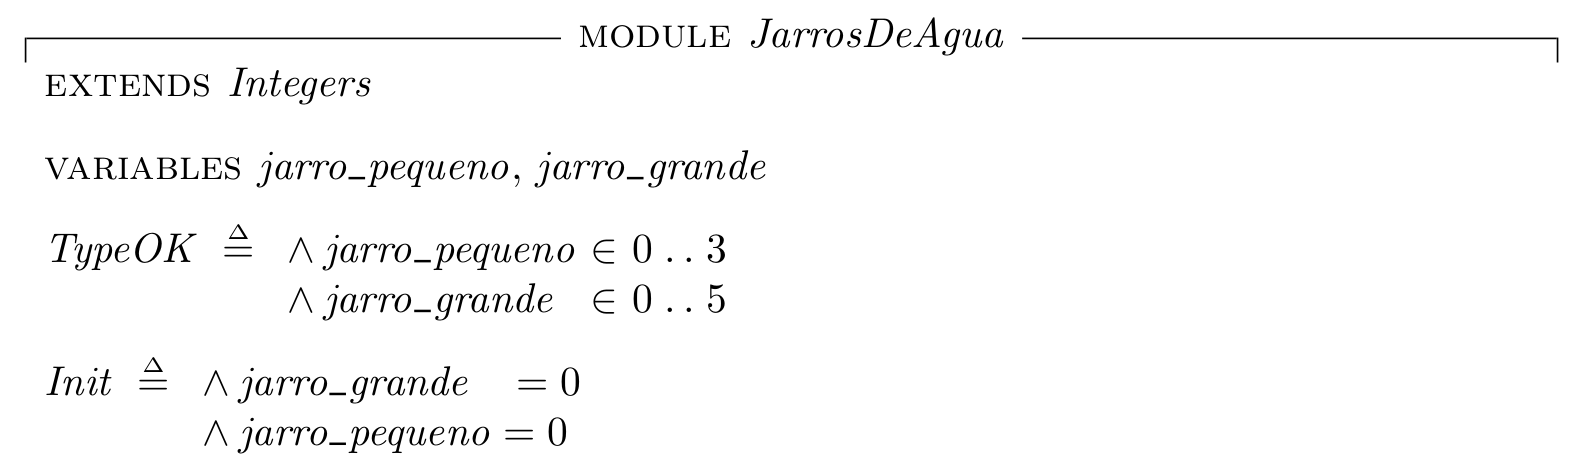
\includegraphics[width=0.9\textwidth]{JarrosP1.png}\\

         \TEqD\ (\texttt{MOD})\\

         \progfigmed{
         defmodule JarrosDeAgua do\\
         ~~require Oracle\\
         ~~@oracle spawn(Oracle, :listen, [])\\
         ~~ ...\\
         end\\
         \\
         JarrosDeAgua.main(\\
         ~~\%\{\\
         ~~~~jarro\_grande: 0,\\
         ~~~~jarro\_pequeno: 0\\
         ~~\}\\
         )
         }
        
       \end{array}$
     }}
   \caption{Tradução do módulo Jarros de Água}
   \label{fig:jarros-ex-mod}
 \end{figure}

 \begin{figure}[h]
  \centering
  {\fbox{
      $\begin{array}{c}

         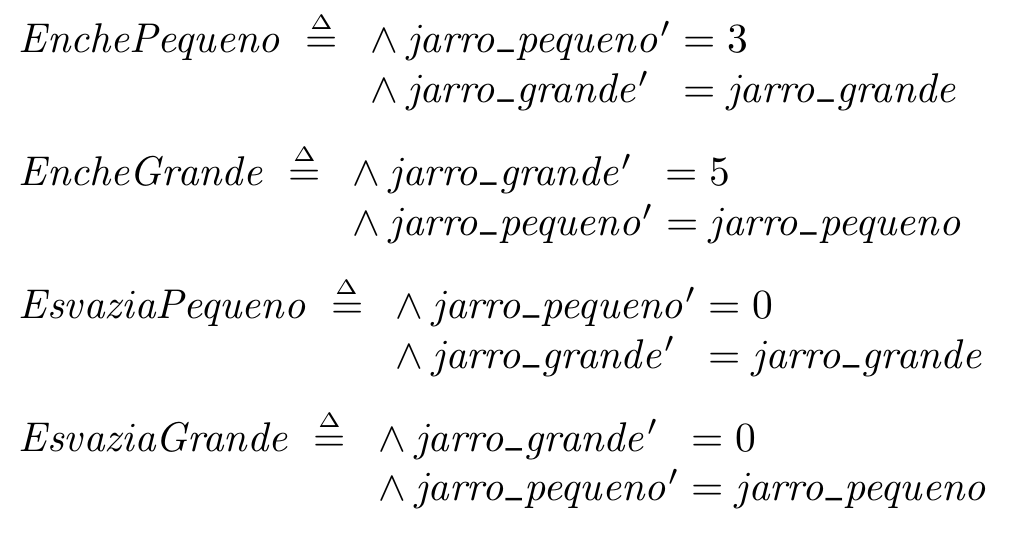
\includegraphics[width=0.6\textwidth]{JarrosP2.png}\\

         \TEqD\ (\texttt{DEF})\\

         \progfigmed{
         def enche\_pequeno\_condition(variables) do\\
         ~~True\\
         end\\\\
         def enche\_pequeno(variables) do\\
         ~~\%\{\\
         ~~~~jarro\_pequeno: 3,\\
         ~~~~jarro\_grande: variables[:jarro\_grande]\\
         ~~\}\\
         end\\
         ...
         }

       \end{array}$
     }}
   \caption{Tradução das definições simples dos Jarros de Água}
   \label{fig:jarros-ex-def1}
 \end{figure}

 \begin{figure}[h]
  \centering
  {\fbox{
      $\begin{array}{c}

         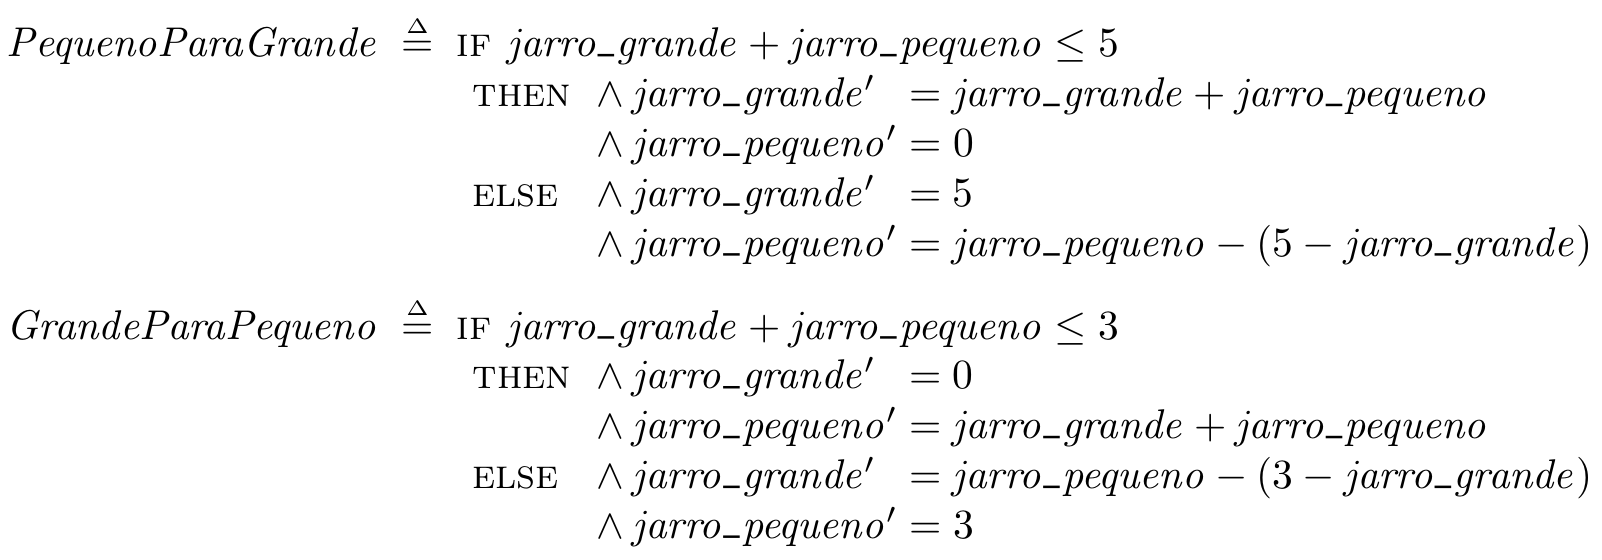
\includegraphics[width=0.9\textwidth]{JarrosP3.png}\\

         \TEqD\ (\texttt{DEF})\\

         \progfig{
         def pequeno\_para\_grande\_condition(variables) do\\
         ~~if variables[:jarro\_grande] + variables[:jarro\_pequeno] \textless{}= 5 do\\
         ~~~~True\\
         ~~else\\
         ~~~~True\\
         ~~end\\
         end\\
         \\
         def pequeno\_para\_grande(variables) do\\
         ~~if variables[:jarro\_grande] + variables[:jarro\_pequeno] \textless{}= 5 do\\
         ~~~~\%\{\\
         ~~~~~~jarro\_grande:\ variables[:jarro\_grande] +\\
         ~~~~~~~~variables[:jarro\_pequeno],\\
         ~~~~~~jarro\_pequeno:\ 0\\
         ~~~~\}\\
         ~~else\\
         ~~~~\%\{\\
         ~~~~~~jarro\_grande:\ 5,\\
         ~~~~~~jarro\_pequeno:\ variables[:jarro\_pequeno] -\\
         ~~~~~~~~(5 - variables[:jarro\_grande])\\
         ~~~~\}\\
         ~~end\\
         end\\
         ...
         }
       \end{array}$
     }}
   \caption{Tradução das definições com condicionais dos Jarros de Água}
   \label{fig:jarros-ex-def2}
 \end{figure}

 \begin{figure}[h]
  \centering
  {\fbox{
      $\begin{array}{c}

         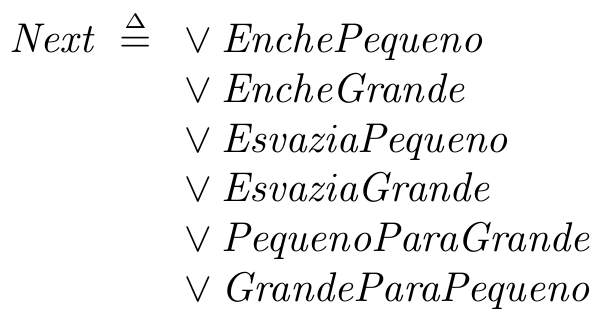
\includegraphics[width=0.4\textwidth]{JarrosP4.png}\\

         \TEqD\ (\texttt{NEXT})\\

         \progfig{
         def main(variables) do\\
         ~~IO.puts (inspect variables)\\
         \\
         ~~main(\\
         ~~~~decide\_action(\\
         ~~~~~~List.flatten([\\
         ~~~~~~~~\%\{\\
         ~~~~~~~~~~action: "EnchePequeno()",\\
         ~~~~~~~~~~condition: enche\_pequeno\_condition(variables),\\
         ~~~~~~~~~~state: enche\_pequeno(variables)\\
         ~~~~~~~~\},\\
         ~~~~~~~~\%\{\\
         ~~~~~~~~~~action: "EncheGrande()",\\
         ~~~~~~~~~~condition: enche\_grande\_condition(variables),\\
         ~~~~~~~~~~state: enche\_grande(variables)\\
         ~~~~~~~~\},\\
         ~~~~~~~~...\\
         ~~~~~~])\\
         ~~~~)\\
         ~~)\\
         end
         }
       \end{array}$
     }}
   \caption{Tradução da função de próximo estado para os Jarros de Água}
   \label{fig:jarros-ex-next}
 \end{figure}

A especificação do sistema de Jarros de Água contém poucos elementos e é ideal
para exemplificar os mapeamentos mais básicos. A tradução do módulo inicia pela
aplicação da regra (\texttt{MOD}) demonstrada na Figura \ref{fig:jarros-ex-mod}.
A especificação não apresenta constantes, descartando a necessidade de aplicar a
regra (\texttt{CONST}).

A definição $TypeOK$ é uma invariante da especificação e, apesar de apresentar
um predicado válido, não representa valor algum para a execução e, portanto, foi
manualmente descartado. O estado inicial definido por $Init$ - conforme identificado como
parâmetro da tradução - e gera a chamada para \texttt{JarrosDeAgua.main}
apresentada. Os parâmetros com os quais a função é chamada são resultado da
aplicação das regras (\texttt{INIT-AND}) e (\texttt{INIT-EQ}), e pela mesma
agregação de literais feita para ações, que omite chamadas de \texttt{Map.merge}
e foi exemplificada na Seção \ref{sec:regras}.

No interior do módulo, são listadas as definições. As definições dessa
especificação se agrupam em duas formas similares: a primeira contendo apenas
modificações de variáveis, e a segunda apresentando uma expressão \texttt{IF}. A
Figura \ref{fig:jarros-ex-def1} demonstra o resultado da tradução para
definições do primeiro grupo, apresentado também na figura.

O segundo grupo de definições traduz para uma condicional de Elixir conforme a
Figura \ref{fig:jarros-ex-def2}. Destaca-se a diferença entre uma ação com uma
expressão \texttt{IF} e um predicado, que gera uma condição. A expressão
$jarro\_grande + jarro\_pequeno \lte 5$ não é uma condição para a execução da
ação, a ação pode ser ativada a qualquer momento. Essa expressão apenas altera
os valores a serem atribuídos às variáveis do próximo estado.

Para ambos os grupos de definições, a regra (\texttt{AND}) é usada para agregar
as condições e ações encontradas para cada linha da definição. Em nenhuma
definição há condições, resultando portanto em uma lista vazia que será
compreendida como \texttt{True}. Todas as ações utilizam o operador
\textit{primed}, e portanto são traduzidas através da regra (\texttt{ACT-PRIM}).

Por fim, a definição de próximo estado por $Next$, assim como $Init$ identificado através
de um parâmetro do tradutor, é traduzida pela regra (\texttt(Next)) conforme a
Figura \ref{fig:jarros-ex-next}. A função \texttt{main} é recursiva, sempre
chamando ela mesma com o próximo estado, sempre imprimindo o estado com que foi
chamada para que seja possível acompanhar suas alterações. A definição $Next$
apresenta ações separadas pelo operador $\lor$, e portanto requer uma decisão.
Como discutido na Seção \ref{sec:decisao}, a decisão é delegada para a função
\texttt{decide\_action}, que recebe uma lista com informações sobre as possíveis
ações.

Essa lista de ações é exemplificada com as informações para as duas primeiras
ações disponíveis, onde a chave \texttt{action} tem como valor uma identificação
daquela ação, \texttt{condition} chama a função de condição que irá retornar se
ela está satisfeita, e \texttt{state} informa qual o novo estado caso a decisão
seja aquela ação.

\subsubsection{Execução}

Devido à ausência de condições, cada mudança de estado - isto é, cada chamada da
função \texttt{main} - exige uma escolha, de forma que a maior parte do
funcionamento do código gerado dependerá da implementação do oráculo. Supondo um
oráculo que escolha sempre uma ação aleatória entre as enviadas a ele, a
execução dos jarros de água se dará pela alteração aleatória de quantidade de
água nos jarros, porém sempre respeitando as mudanças especificadas.

Outra implementação possível para o oráculo é a leitura de alguma entrada que
determine a ação a ser tomada. Com essa implementação, o resultado da execução
pode ser entendido como um jogo ou simulação, onde algum usuário determina uma
ação e observa um resultado, de forma que as restrições impostas pela
especificação funcionem como regras que limitam as operações a serem feitas pelo
usuário.

\subsection{Protocolo de efetivação em duas fases}





